\chapter{Prototype vs.\ Product \& Selective Prototyping}
\label{ch3}

Every engineering team has a finite budget of time, money, and attention.
The moment you begin building something --- anything --- you are spending that
budget.
The central question of this chapter is not \emph{how} to prototype, but
\emph{what} to prototype and \emph{why}.
A well-targeted prototype teaches you something you could not learn any other
way and reduces the risk of discovering an expensive flaw later.
A poorly targeted prototype keeps the team busy, drains the budget, and leaves
the real unknowns untouched.

By the end of this chapter you will be able to draw a clear line between the
seven subsystems of your IoT sorting system: four demand a hands-on prototype;
three do not.
The discipline of drawing that line --- and defending it --- is the core skill
this chapter builds.

\section*{Learning Objectives}
\begin{enumerate}
  \item Contrast a prototype and a product across goals, standards, and
        lifecycle obligations.
  \item Separate intrinsic value (knowledge, risk reduction) from extrinsic
        value (artifact quality) in a practical decision.
  \item Apply the cost-of-change heuristic to justify front-loading design
        decisions.
  \item Classify subsystems as either ``prototype'' or ``specify-and-trust''
        using defined criteria.
\end{enumerate}

% ============================================================
\section{Goals and Standards: Learning vs.\ Reliability}
\label{sec:ch3-goals-and-standards}
% ============================================================

Start with a question most teams skip: what is the object you are building
\emph{for}?

A \textbf{prototype}\index{prototype} is an artifact whose primary purpose is
to generate knowledge.
You build it to answer a question, reduce uncertainty, or demonstrate that a
physical principle works at the scale and under the conditions that matter for
your product.
The prototype may be ugly, fragile, hand-wired, held together with cable ties,
and powered by a bench supply.
None of that matters as long as it answers the question it was built to answer.
The moment it does, its job is done.

A \textbf{product}\index{product} is an artifact whose primary purpose is to
deliver reliable value to a customer across the full lifecycle of use.
It must meet regulatory requirements, survive handling and shipping, operate
within specified environmental limits, and be maintainable and repairable by
people who were not in the room when it was designed.
Reliability, not learning, is the governing criterion.

This distinction shapes every design decision that follows.
Consider the two objects side by side across four dimensions.

\paragraph{Goals.}
A prototype's goal is epistemic: you want to know something you do not yet
know.
Is the ML inference fast enough on the target MCU?
Does the servo divert reliably at 6~items per minute under a 200~g load?
A product's goal is operational: deliver the specified function to the customer
on schedule, within cost, and without failure in the field.

\paragraph{Standards.}
Prototypes are typically exempt from --- or at least not yet subject to ---
formal certification requirements.
You do not CE-mark a breadboard.
Products must meet all applicable standards in every jurisdiction where they
are sold: electrical safety, EMC, RoHS compliance, industry-specific standards
for the operating environment.
For your sorting subsystem shipped under a Hardware-as-a-Service (HaaS) model,
this means your final product must meet the standards of a production floor,
not a university lab.

\paragraph{Lifecycle obligations.}
A prototype has no lifecycle obligation beyond the experiment it supports.
When you have your answer, you can dismantle it.
A product carries a service life: firmware updates, spare parts, warranty
claims, end-of-life disposal.
Designing for lifecycle obligations adds cost and complexity that is
inappropriate --- and wasteful --- to impose on a prototype.

\paragraph{Failure modes.}
Prototype failure is valuable.
If the sensor field of view is too narrow and items slide past unclassified,
you have learned exactly what you needed to learn, cheaply.
Product failure has consequences: warranty claims, customer downtime,
reputational damage, potential liability.
The standards a product must meet are precisely the standards required to make
failure improbable under foreseeable conditions.

\textbf{Intrinsic value}\index{intrinsic value} is the knowledge and risk
reduction produced by building and testing an artifact, regardless of whether
the artifact itself is ever used again.
\textbf{Extrinsic value}\index{extrinsic value} is the value of the artifact
as a deliverable --- its functional quality, finish, reliability, and
compliance.

A prototype optimizes for intrinsic value.
A product must optimize for extrinsic value.
The practical mistake most teams make is to apply product-level quality
expectations to prototype work --- spending days on a clean PCB layout before
the core algorithm has been validated --- or, conversely, to ship a
prototype-quality object to a customer and call it a product.

\paragraph{In Practice.}
At your twelve-person start-up, the distinction between prototype and product
is under constant pressure.
Investors want to see polished demos; customers want reliable hardware;
engineers want to close tickets.
The discipline is to keep the question clear at all times: are we building
this to \emph{learn} something, or to \emph{deliver} something?
The answer determines the standard you hold it to, the time you spend on it,
and when you are done.


% ============================================================
\section{Selective Prototyping: Target High Risk and Uncertainty}
\label{sec:ch3-selective-prototyping}
% ============================================================

Given that a prototype costs time and money, the decision to prototype a
subsystem is a resource allocation decision.
\textbf{Selective prototyping}\index{selective prototyping} is the discipline
of directing prototype effort only at the subsystems where the cost of
remaining uncertain exceeds the cost of building and testing an artifact.

The decision logic is straightforward and can be expressed as three questions.

\begin{enumerate}
  \item \textbf{Is the subsystem novel?}\index{novelty criterion}
        Has your team built and validated this combination of components,
        firmware, and mechanical arrangement before?
        If not, you have a knowledge gap that a prototype can close.
  \item \textbf{Is the subsystem uncertain?}\index{uncertainty criterion}
        Does the subsystem's performance under your specific conditions depend
        on factors you cannot fully resolve from datasheets and first
        principles?
        Mechanical resonance under dynamic load, ML inference latency on a
        specific MCU, Wi-Fi packet loss rates in a metal-walled production
        environment --- these are inherently empirical questions.
  \item \textbf{Is failure high-consequence?}\index{consequence criterion}
        If the subsystem fails or underperforms, does it compromise the core
        value proposition or create safety, financial, or customer-relationship
        risk that is disproportionate?
\end{enumerate}

If the answer to any of these questions is ``yes,'' the subsystem is a
prototype candidate.
If the answer to all three is ``no,'' the subsystem is a candidate for
\textbf{specify-and-trust}\index{specify-and-trust}: you select a
well-characterized off-the-shelf (OTS) component, confirm it meets your
requirements from the datasheet, and integrate it without building a
prototype.

Figure~\ref{fig:ch3-selective-decision} shows this decision flow as a diagram.
Work through it for each subsystem in your design, and record the decision with
a one-sentence justification.
The justification is not bureaucratic overhead --- it is the record that tells
the next engineer (or future you) why a prototype was or was not built, so the
decision can be revisited if requirements change.

\begin{figure}[htbp]
  \centering
  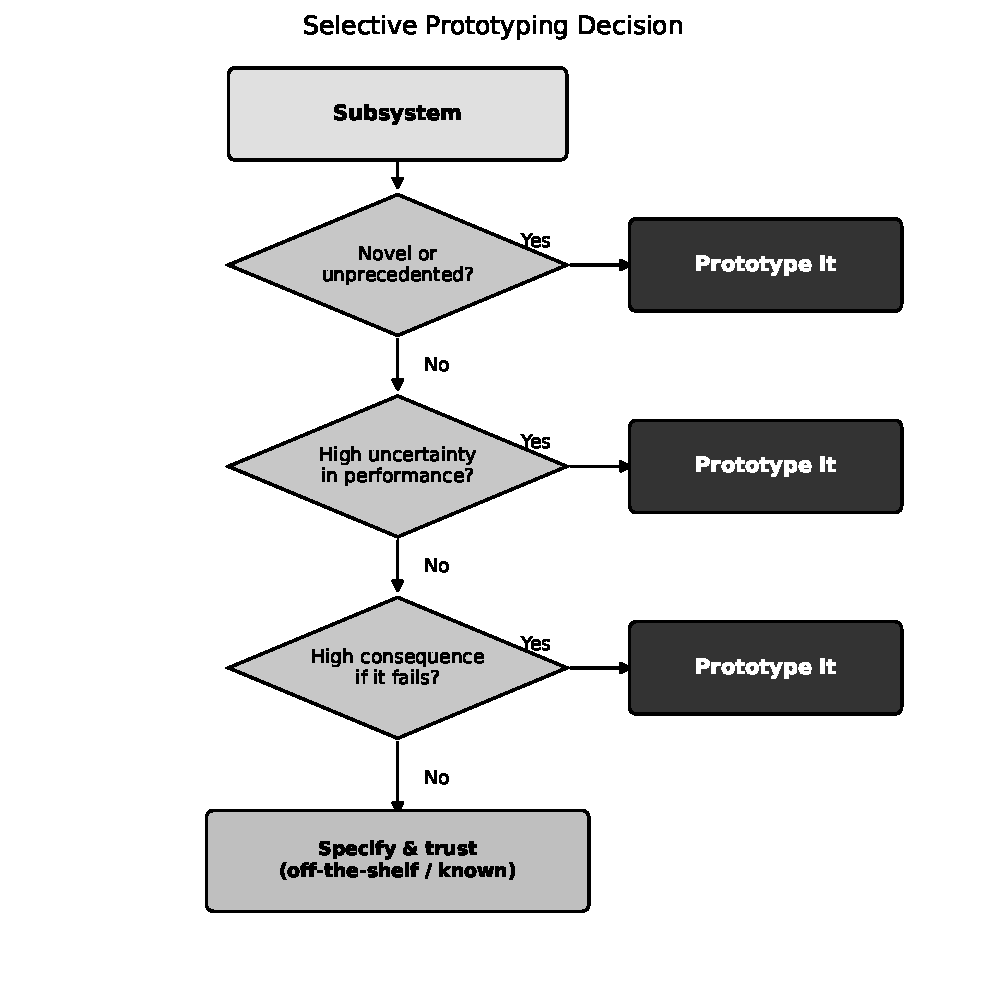
\includegraphics[width=0.85\textwidth]{images/fig_02_selective_decision.pdf}
  \caption{Decision flow for classifying a subsystem as prototype or
           specify-and-trust. Only novel, uncertain, or high-consequence
           subsystems justify the effort of building a prototype.}
  \label{fig:ch3-selective-decision}
\end{figure}

\subsection*{What ``Specify-and-Trust'' Actually Means}

Choosing to specify-and-trust is not the same as choosing to ignore.
It means you invest your engineering effort in writing a precise requirement
--- a performance specification with numerical bounds --- rather than in
building and testing an artifact.
You then select a component whose datasheet confirms it meets that
specification, document that selection decision, and move on.

For the OTS conveyor belt module in your sorting subsystem, ``specify and
trust'' means you write: ``Belt conveyor module shall transport items at
$6 \pm 0.5$~items per minute at 200~g average item mass, with a mean time
between failures (MTBF) $\geq 2{,}000$~hours.''
You select a module whose datasheet meets that spec, log the part number, and
integrate it.
You do not spend a week running test items over a borrowed belt to confirm what
the supplier already guarantees.

The budget you save goes directly to the subsystems that need it: the sensor
pipeline, the actuator timing, the firmware, and the MQTT connectivity.

\paragraph{In Practice.}
Teams often prototype familiar subsystems first because the work is
comfortable and fast.
Resist this.
The sensor pipeline is the riskiest subsystem in your design, and it is the
last thing you want to discover is broken at the integration stage.
The decision of \emph{what} to prototype is more important than \emph{how
well} any individual prototype is executed.


% ============================================================
\section{The Cost of Changing a Design Later}
\label{sec:ch3-cost-of-change}
% ============================================================

The strongest argument for front-loading prototype work --- for doing it early
and systematically --- is the cost of change.
Design flaws do not get cheaper to fix as a project progresses.
They get dramatically more expensive.

\subsection*{The Cost-of-Change Heuristic}

Let $s$ denote the \textbf{project stage}\index{project stage} as an integer:

\begin{center}
\begin{tabular}{cl}
\toprule
$s$ & Stage \\
\midrule
0 & Concept \\
1 & Design \\
2 & Build (Prototype / Pre-production) \\
3 & Production \\
\bottomrule
\end{tabular}
\end{center}

The \textbf{cost-of-change heuristic}\index{cost-of-change heuristic} states
that the cost of fixing a given design flaw at stage $s$ is approximately:

\begin{equation}
  C_{\text{change}}(s) \approx C_0 \cdot 10^{\,s}
  \label{eq:ch3-cost-of-change}
\end{equation}

where $C_0$\index{$C_0$, baseline cost} is the cost of fixing the same flaw at
the Concept stage ($s = 0$).
The exponent reflects the compounding difficulty: each stage adds committed
procurement, tooling, testing infrastructure, and --- in production ---
physical units that must be reworked or scrapped.

This heuristic originates in empirical studies of software and hardware
projects from the 1970s onward and has been reproduced across aerospace,
consumer electronics, and industrial systems.
The exact multiplier varies by industry; the order-of-magnitude-per-stage
relationship is robust.

\subsection*{Worked Table}

Set $C_0 = \$50$~CAD, roughly one engineering hour at a start-up billing rate.

\begin{table}[htbp]
  \centering
  \caption{Cost to fix the same design flaw at each project stage, with
           $C_0 = \$50$~CAD.}
  \label{tab:ch3-cost-of-change}
  \begin{tabular}{clrr}
    \toprule
    $s$ & Stage & Formula & Cost (CAD) \\
    \midrule
    0 & Concept     & $\$50 \times 10^0$ & \$50 \\
    1 & Design      & $\$50 \times 10^1$ & \$500 \\
    2 & Build       & $\$50 \times 10^2$ & \$5{,}000 \\
    3 & Production  & $\$50 \times 10^3$ & \$50{,}000 \\
    \bottomrule
  \end{tabular}
\end{table}

The savings from finding a flaw at the Design stage rather than at Production
is:

\begin{align}
  \Delta C &= C_{\text{change}}(3) - C_{\text{change}}(1) \notag \\
           &= C_0 \bigl(10^3 - 10^1\bigr) \notag \\
           &= \$50 \times 990 \notag \\
           &= \$49{,}500
  \label{eq:ch3-savings}
\end{align}

That is the value created by a prototype that catches one flaw before
production begins.
At a BOM cost target of \$480~CAD per unit and a twelve-person team, finding
even a single sensor-integration flaw early pays for many hours of prototype
work.

Figure~\ref{fig:ch3-cost-of-change} illustrates this escalation graphically.
The vertical axis is logarithmic; the relationship is linear on that scale,
which makes the exponential growth viscerally clear.

\begin{figure}[htbp]
  \centering
  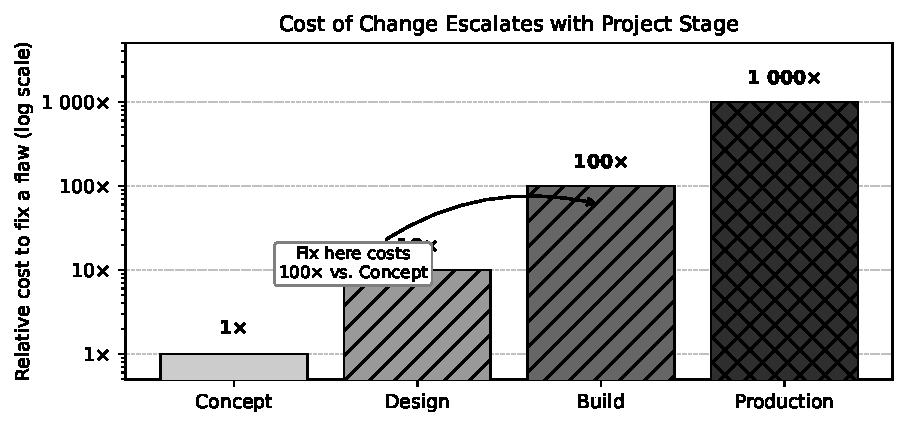
\includegraphics[width=0.85\textwidth]{images/fig_01_cost_of_change.pdf}
  \caption{Cost of fixing a design flaw escalates by roughly one order of
           magnitude per project stage. A flaw caught at the Concept stage
           costs $C_0$; the same flaw at Production costs $1{,}000\,C_0$.}
  \label{fig:ch3-cost-of-change}
\end{figure}

\subsection*{Implications for Prototype Targeting}

Equation~\eqref{eq:ch3-cost-of-change} does not tell you which subsystem to
prototype.
It tells you \emph{why} the decision matters.
Combine it with the three selectivity criteria from
Section~\ref{sec:ch3-selective-prototyping}: a subsystem that is novel,
uncertain, and high-consequence is precisely the subsystem most likely to
harbor a flaw that, if undetected until Production, will cost $10^3 C_0$ to
fix.

The rational response is to prototype it now, at the cost of
$10^0 C_0$ to $10^1 C_0$, and find the flaw while it is still cheap.

\paragraph{In Practice.}
A common objection is ``we will catch it during integration testing.''
Integration testing is stage~2 (Build) in the framework above.
Finding a sensor field-of-view problem at integration costs \$5{,}000, not
\$50.
The flaw was always findable earlier; the question is whether you built the
right prototype to find it.


% ============================================================
\section{Known and Off-the-Shelf Subsystems: Specify and Trust}
\label{sec:ch3-specify-and-trust}
% ============================================================

Not every subsystem is a source of risk.
A mature, well-documented off-the-shelf (OTS) module has been designed,
tested, and certified by an organization with more relevant experience than
your team.
The manufacturer has already run thousands of hours of life testing.
The datasheet encodes the results of that testing as specifications you can
use directly.

\textbf{Off-the-shelf}\index{off-the-shelf (OTS)} subsystems are appropriate
candidates for specify-and-trust when all of the following hold:

\begin{enumerate}
  \item The performance parameters you need are \emph{fully specified} in the
        manufacturer's datasheet or product bulletin.
  \item Your operating conditions (load, temperature, supply voltage,
        duty cycle) fall within the specified operating range with adequate
        margin.
  \item Failure of the subsystem is either detectable before it affects output
        quality, or its consequence is low enough that reactive replacement is
        acceptable.
  \item The subsystem does not interact in a novel way with other subsystems
        in your design.
\end{enumerate}

When all four conditions hold, you can write a requirement, confirm the
datasheet match, log the decision, and redirect your prototype budget.

\subsection*{Writing the Requirement}

``Specify and trust'' begins with a clear requirement, not with browsing a
catalogue.
The requirement defines what the subsystem must do in your system, expressed
in terms your team can verify from a datasheet.

For the 5~V / 12~V power supply in the sorting subsystem, a well-formed
requirement might be:

\begin{quote}
  The power supply shall provide 5~V~DC $\pm$5\% at up to 3~A and 12~V~DC
  $\pm$5\% at up to 2~A simultaneously, with output ripple $\leq 50$~mV
  peak-to-peak, certified to UL 60950-1 or equivalent, operating at ambient
  temperatures from $0{^\circ}$C to $50{^\circ}$C.
\end{quote}

A switched-mode PSU from any reputable industrial supplier will meet this
specification.
You confirm the datasheet, log the part number, and move on.
No prototype is needed.

\paragraph{Common Pitfalls.}
\begin{itemize}
  \item \textbf{Over-specifying OTS components.}\index{over-specification}
        Writing requirements more stringent than your system actually needs
        narrows the supplier pool unnecessarily and drives up cost.
        Specify what you need; trust the datasheet to confirm the rest.
  \item \textbf{Under-specifying integration conditions.}
        An OTS conveyor belt module rated for 200~g loads will fail if your
        items occasionally reach 350~g.
        Specify the \emph{actual} worst-case operating conditions, including
        margin, not the nominal design point.
  \item \textbf{Skipping the datasheet confirmation step.}
        ``Specify and trust'' means trust the datasheet, not trust the product
        name.
        The confirmation step --- reading the datasheet and recording that it
        meets your requirement --- is not optional.
\end{itemize}


% ============================================================
\section*{Worked Example: IoT Sorting Subsystem Classification}
\label{sec:ch3-worked-example}
% ============================================================

Apply the selective prototyping framework to the seven subsystems of the IoT
robotic sorting system.
Recall from Chapter~2 that the central question is: can a sub-\$500 BOM sorter
achieve $\geq$95\% sort accuracy at 6~items per minute with reliable MQTT
connectivity?
The Level~2 (proof-of-concept) fidelity decision commits you to breadboard
electronics, a 3D-printed bracket, and firmware with data logging.

\subsection*{Subsystem Classification Table}

Table~\ref{tab:ch3-classification} applies the three criteria to each
subsystem and records the resulting decision.

\begin{table}[htbp]
  \centering
  \caption{Selective prototyping classification for the IoT robotic sorting
           subsystem. Four subsystems require prototype effort; three are
           appropriate for specify-and-trust.}
  \label{tab:ch3-classification}
  \small
  \begin{tabular}{p{3.0cm} c c c p{1.8cm} p{4.5cm}}
    \toprule
    Subsystem &
      Novel? &
      Uncertain? &
      High-cons.? &
      Decision &
      Justification \\
    \midrule
    Sort sensor (camera + ML inference)
      & Yes & Yes & Yes
      & \textbf{Prototype}
      & Novel ML pipeline; accuracy uncertain; misclassification is the core
        risk \\[4pt]
    Divert actuator (servo + gate mechanism)
      & Partial & Yes & Yes
      & \textbf{Prototype}
      & Mechanical timing under load is unproven; failure stops sorting \\[4pt]
    Embedded MCU + firmware
      & Yes & Yes & Yes
      & \textbf{Prototype}
      & Custom firmware and sensor integration; timing and power unknown \\[4pt]
    MQTT / Wi-Fi connectivity
      & No & Yes & Yes
      & \textbf{Prototype}
      & Known protocol but real-time reliability on production floor is
        unproven \\[4pt]
    Conveyor belt (OTS module)
      & No & No & No
      & Specify \& trust
      & Standard industrial conveyor; datasheet specs sufficient \\[4pt]
    5~V / 12~V power supply (OTS PSU)
      & No & No & No
      & Specify \& trust
      & Standard switched-mode PSU; certified component \\[4pt]
    Structural frame (3D-printed PLA)
      & No & No & No
      & Specify \& trust
      & Low-consequence geometry; standard material; no structural
        certification required \\
    \bottomrule
  \end{tabular}
\end{table}

The result: \textbf{4 subsystems to prototype} (sort sensor, divert actuator,
MCU/firmware, MQTT integration); \textbf{3 to specify-and-trust} (conveyor
belt, PSU, structural frame).
This classification feeds directly into the risk register you will build in
Chapter~4.

\subsection*{Cost-of-Change Calculation: Two Representative Flaws}

Apply Equation~\eqref{eq:ch3-cost-of-change} to two concrete flaws that could
reasonably affect the sorting subsystem.

\paragraph{Flaw~A: Sort sensor field of view too narrow.}
The camera is mounted at a fixed height with a fixed lens.
During prototype testing you discover that items wider than 80~mm pass
partially outside the field of view, causing the ML model to misclassify them.

\medskip
\noindent\textit{Detected at the Design stage} ($s = 1$):
\begin{equation}
  C_{\text{change}}(1) = \$50 \times 10^1 = \$500
  \label{eq:ch3-flaw-a-design}
\end{equation}
Remediation: redesign the bracket to lower the camera by 30~mm, reprint the
PLA bracket (cost: 4~hours of engineering time, one print job), rerun the
accuracy test.
Total cost is roughly one day of work.

\medskip
\noindent\textit{Detected at the Production stage} ($s = 3$):
\begin{equation}
  C_{\text{change}}(3) = \$50 \times 10^3 = \$50{,}000
  \label{eq:ch3-flaw-a-production}
\end{equation}
Remediation: retool the injection-moulded housing (new mould insert,
minimum 6-week lead time), re-certify the modified assembly, rework or scrap
50~units already built.
At a unit BOM of \$480 and 50~units, scrap alone approaches \$24{,}000;
the tooling and re-certification absorb the remainder.

\paragraph{Saving from early detection.}
\begin{align}
  \Delta C &= C_{\text{change}}(3) - C_{\text{change}}(1) \notag \\
           &= \$50{,}000 - \$500 \notag \\
           &= \$49{,}500
  \label{eq:ch3-saving-flaw-a}
\end{align}

\paragraph{Flaw~B: MQTT reconnection loop blocks sensor pipeline.}
The firmware's Wi-Fi reconnection routine holds a mutex that the sensor
sampling task also requires.
On reconnect, sensor sampling pauses for up to 3~seconds, during which items
pass the camera unclassified.

\medskip
\noindent\textit{Detected at the Design stage} ($s = 1$, during prototype
firmware testing with a simulated RF interference event):

\begin{equation}
  C_{\text{change}}(1) = \$50 \times 10^1 = \$500
  \label{eq:ch3-flaw-b-design}
\end{equation}
Remediation: refactor the reconnection handler to operate on a dedicated task
with its own stack, remove the shared mutex.
Estimated effort: one sprint, two engineers, largely confined to the firmware
module.

\medskip
\noindent\textit{Detected at the Production stage} ($s = 3$):

\begin{equation}
  C_{\text{change}}(3) = \$50 \times 10^3 = \$50{,}000
  \label{eq:ch3-flaw-b-production}
\end{equation}
Remediation: firmware update requires regression testing of all embedded
functionality, re-validation of the MQTT reliability specification across
representative production-floor RF conditions, customer notification, potential
SLA penalty under the HaaS contract.

\medskip
Both calculations reinforce the same conclusion: the most economically
rational place to discover and fix design flaws is as early as possible.
The Level~2 proof-of-concept prototype, built for a few hundred dollars in
components and a few weeks of engineering time, is the instrument that makes
that early discovery possible.

\paragraph{In Practice.}
At the HaaS pricing of \$1{,}200~CAD per unit and a gross margin of 60\%, each
unit contributes \$720~CAD toward overhead and profit.
A firmware flaw found at Production that requires reworking 50~units
eliminates the entire gross margin contribution of 69~units --- nearly three
months of sales at the early-stage volumes typical of a twelve-person start-up.
Prototype investment is not a cost; it is margin protection.


% ============================================================
\section*{Common Pitfalls}
\label{sec:ch3-pitfalls}
% ============================================================

\paragraph{Common Pitfalls.}
\begin{description}
  \item[Prototyping the easy subsystem first.]
        It is tempting to begin with the conveyor belt or the power supply
        because those subsystems are well understood and progress feels fast.
        Resist this.
        Spend your first prototype sprint on the sort sensor pipeline.
        That is where your central hypothesis lives --- whether a sub-\$500
        BOM can achieve 95\% accuracy --- and it is the only place where
        prototype results can confirm or refute the viability of the product.
        Comfort is not a valid criterion for prototype sequencing.
        Risk is.

  \item[Calling unplanned tinkering ``iteration.'']
        Iteration is a documented cycle: you state a hypothesis, build the
        minimum artifact needed to test it, run the test, measure against a
        predefined criterion, and update the design based on what you learned.
        Tinkering --- adjusting parameters without a recorded baseline,
        rerunning a test without changing the design, ``trying things'' without
        a clear success criterion --- consumes time and produces no defensible
        knowledge.
        Every prototype run should be linked to a hypothesis from the
        specification document.
        If you cannot state the hypothesis in one sentence before you start the
        test, you are not iterating; you are tinkering.

  \item[Letting prototype quality inflate toward product quality.]
        Once a prototype validates a subsystem, the pressure to ``clean it up''
        before moving on is real.
        A clean, well-labelled PCB feels better than a breadboard.
        Resist the impulse unless a specific requirement --- mechanical
        robustness, EMC pre-scan, thermal testing --- demands it.
        The purpose of the Level~2 prototype is to answer the central question,
        not to produce a product.
        Over-finishing a prototype is borrowed time that the product phase will
        demand back.

  \item[Confusing specify-and-trust with specify-and-forget.]
        A requirement written at the start of the project may cease to be
        correct if the design evolves.
        If your item mix changes and maximum item mass increases from 200~g to
        350~g, revisit every OTS selection that was made under the original
        assumption.
        ``Specify and trust'' is not a permanent waiver; it is a standing
        decision that must be revisited when the requirements it was based on
        change.
\end{description}


% ============================================================
\section*{End-of-Chapter Artifact: Subsystem Classification Table}
\label{sec:ch3-artifact}
% ============================================================

The deliverable for this chapter is a completed subsystem classification table
for your own project, structured identically to
Table~\ref{tab:ch3-classification}.
It must contain one row per subsystem with the following columns:

\begin{center}
\begin{tabular}{lp{7cm}}
\toprule
Column & Content \\
\midrule
Subsystem & Name of the subsystem \\
Novel? & Yes / Partial / No \\
Uncertain? & Yes / No \\
High-consequence? & Yes / No \\
Decision & Prototype \emph{or} Specify \& trust \\
Justification & One sentence explaining the decision \\
\bottomrule
\end{tabular}
\end{center}

Every subsystem in your design must appear in the table.
Subsystems classified as ``Prototype'' become candidates for the risk register
in Chapter~4.
Subsystems classified as ``Specify \& trust'' must have a corresponding
documented requirement and a named datasheet that confirms compliance.

For the sorting subsystem, the completed table is
Table~\ref{tab:ch3-classification} above.
The four prototype subsystems --- sort sensor, divert actuator, MCU/firmware,
and MQTT integration --- will each receive a risk entry and a prototype
hypothesis in Chapter~4.
The three specify-and-trust subsystems --- conveyor belt, PSU, and structural
frame --- will each receive a formal requirement and a datasheet citation at
Milestone~1.


% ============================================================
\section*{Summary and Transition}
\label{sec:ch3-summary}
% ============================================================

This chapter established the foundational judgment that separates effective
from ineffective prototype practice: the decision of \emph{what} to prototype.

A prototype optimizes for intrinsic value --- knowledge and risk reduction.
A product optimizes for extrinsic value --- reliability, compliance, and
lifecycle performance.
Conflating the two wastes resources in both directions.

Selective prototyping directs effort at subsystems that are novel, uncertain,
or high-consequence.
Subsystems that fail all three tests are better handled through
specify-and-trust: write a precise requirement, confirm it against a datasheet,
and redirect the saved time to the subsystems that actually need
experimentation.

The cost-of-change heuristic, $C_{\text{change}}(s) \approx C_0 \cdot 10^s$,
quantifies why this matters.
Finding a flaw at the Design stage rather than Production saves approximately
$C_0 \times 990$ --- for a \$50 baseline, that is \$49{,}500.
For a twelve-person start-up operating on thin margins, early flaw detection is
not an engineering nicety; it is a financial necessity.

Applied to the IoT sorting subsystem, the framework identifies four subsystems
to prototype (sort sensor, divert actuator, MCU/firmware, MQTT integration) and
three to specify-and-trust (conveyor belt, PSU, structural frame).

\medskip
\noindent\textbf{Transition to Chapter~4.}
With the subsystem classification complete, you are ready to formalize what you
know and what you do not.
Chapter~4 introduces the specification document --- the Milestone~1 deliverable
--- and the risk register that will govern your prototype sequencing.
Each of the four prototype subsystems will receive a formal hypothesis, a
measurable success criterion, and a risk priority score.
The three specify-and-trust subsystems will receive finalized requirements and
sourcing decisions.
The structure you have built in this chapter is the direct input to that
process.
